%\section*{User und Rollenmanagement}
\cfoot{Philipp Adler}

\subsubsection{Usermanagment}
Unter dem Begriff Usermanagement versteht sich, dass verwalten und kontrollieren von Benutzerkonten. Es soll dazu dienen jeden registrierten User eindeutig zu identifizieren und zu kontrollieren, ob die monatlichen Raten für einen Pro-Account überwiesen wurden. Außerdem soll die bereits in Anspruch genommene Speicherkapazität überwacht werden. Dazu ist notwendig, dass jeder User durch eine Kombination von Daten, einmalig, unterscheidbar von anderen ist.
\subsubsection{Authentisierung}
Unter Authentisierung versteht man den Nachweis der behaupteten Identität der BenutzerInnen. Im Falle von DSN handelt es sich hierbei um die eindeutige Email-Adresse, welche einmalig im System benutzt wird. Unter der Identität versteht sich die Sicherheit von wem die Information stammt. Jedes handeln eines Benutzers kann jemanden zugewiesen werden.\\
Ein weiterer Identitätspunkt wäre, dass zu geheim haltenden Passwort, welches aus Sicherheitsgründen mindestens 8 Zeichen beinhalten muss. Durch 8 Zeichen möchten wir Cyberkriminelle das Knacken von Passwörtern erschweren. Für die Abschließung der Registrierung müssen die Nutzungsbedingungen akzipiert werden. \grqq{}Allgemeine Geschäftsbedingungen (AGB) sind vertragliche Klauseln, die zur Standardisierung und Konkretisierung von Massenverträgen dienen. Sie werden von einer Vertragspartei einseitig gestellt und bedürfen daher einer bes. Kontrolle, um ihren Missbrauch zu verhindern.\grqq{}\cite{AGB}\\
\cite{VERTEILTE_SYSTEME}\cite{PASSWORT_SCHUTZ}

\begin{figure}[ht]
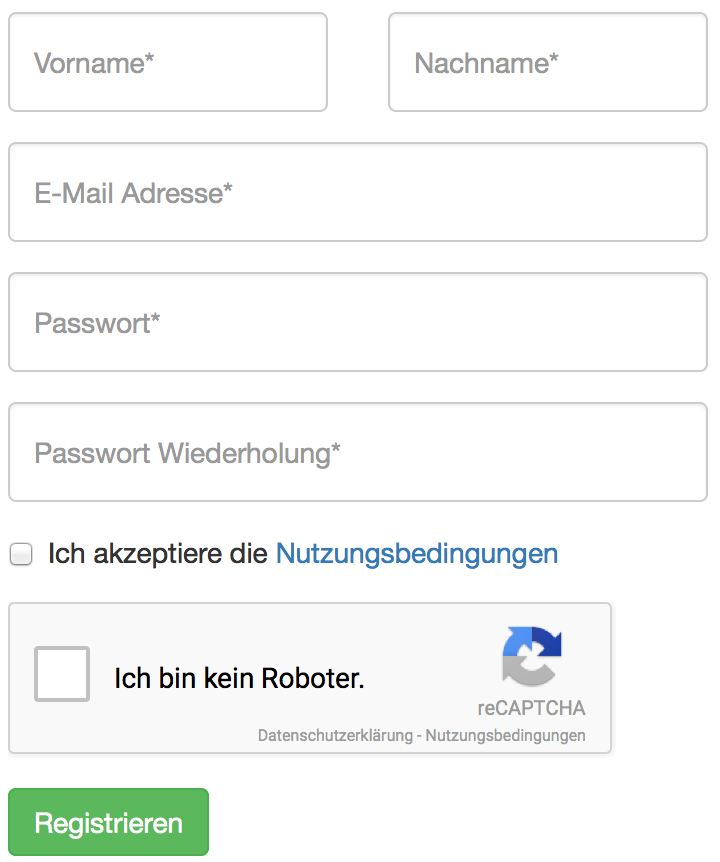
\includegraphics[width=0.35\textwidth]{images/usermanagement/Registrierung}
	\caption{Authentisierung bei DSN}
	\label{fig1}
\end{figure}

Um auszuschließen, dass sich eine Software bzw. ein Roboter einen Account auf DSN erstellt, wird ein Captcha verwendet. Ein Captcha dient zur Sicherheit und soll überprüfen wer die Eingabe tätigte.
Um das Captcha anzuzeigen muss eine JS Lib eingebunden werden \cite{CAPTCHA}.
\begin{lstlisting}[caption={Einbindung der JS-Library Recaptcha}]
<script src="https://www.google.com/recaptcha/api.js?
onload=vcRecaptchaApiLoaded&render=explicit" async defer></script>
<script src="https://cdnjs.cloudflare.com/ajax/libs/angular-recaptcha/2.2.5/
angular-recaptcha.min.js"></script>
\end{lstlisting}

Dannach kann das Captcha einfach wie folgt ins Form eingebunden werden:
\begin{lstlisting}
<div vc-recaptcha key="publicKey"></div>
\end{lstlisting}

publicKey definiert den Public Key des Recaptchas. Dieser wird im Javascript file über \$scope zugewiesen.
Das Captcha wird nach der Benutzereingabe serverseitig validiert. Mit den Daten des Registrierungsformular wird ein weiteres Attribut namens recaptcha erhalten. In diesem steht ein Key der zur Validierung an Google gesendet werden muss. Google möchte zur Validierung den Key, die IP des Users und den Secret App Key. Google gibt dann zurück, ob alles korrekt ablief, also ob es sich bei dem User tatsächlich um ein menschliches Lebewesen handelt. Um die Validierung mehrmals einsetzen zu können, haben wir eine Methode dafür geschrieben:

\begin{lstlisting}
def validate_captcha(recaptcha, ip):
    response = {}
    url = "https://www.google.com/recaptcha/api/siteverify"
    params = {
        'secret': settings.RECAPTCHA_SECRET_KEY,
        'response': recaptcha,
        'remoteip': ip
    }
    verify = requests.get(url, params=params, verify=True)
    verify = verify.json()
    response["status"] = verify.get("success", False)
    if response["status"] == True:
        return True
    else:
        return "Captcha ist nicht valide." 
\end{lstlisting}


Wenn das Captcha gelöst wurde, kann man damit das Form genau ein Mal absenden. Im Falle, dass das Formular nochmals abgesendet werden muss, ist es notwendig das Captcha zurück zu setzen.

\begin{figure}[ht]
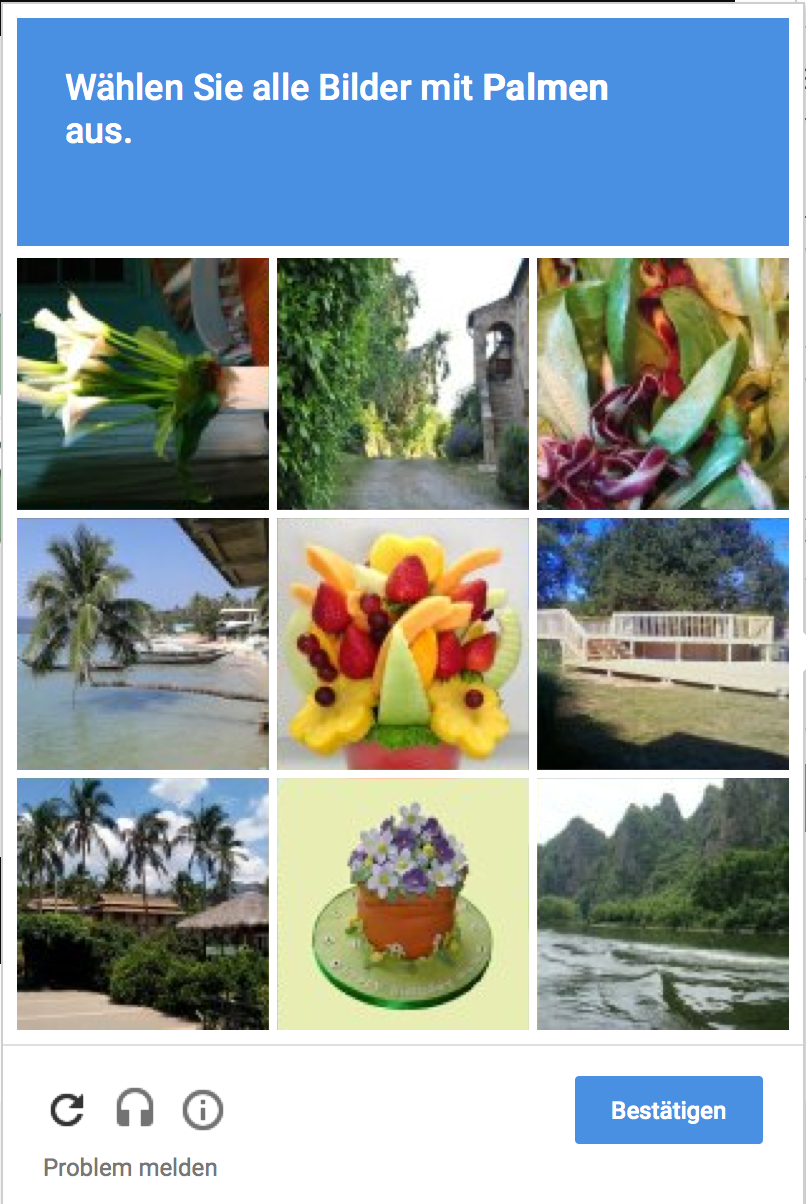
\includegraphics[width=0.35\textwidth]{images/usermanagement/Captcha}
	\caption{Auslösen des Captchas}
	\label{fig2}
\end{figure}

\subsubsection{Datenmodell}
Da Django-Authentifizierungs Funktionalitäten nur für relative DBMS ausgelegt sind, daher für den vorgesehenen Anwendungszweck nicht geeignet sind, mussten Änderungen vorgenommen werden, um die Authentifizierung über MongoDB zu ermöglichen.\\
Nun muss das User-Model, das eben auf Mongo Basis definiert wurde, noch im File models.py erstellt werden. Der Code für das Model wurde aus dem entsprechenden Source-Code von MongoEngine \cite{MONGOENGINE} kopiert und an unseren Anwendungszweck angepasst.
\begin{lstlisting}
class User(Document):
    id = ObjectIdField(unique=True, required=True, primary_key=True)
    email = EmailField(unique=True, required=True)
    first_name = StringField(max_length=30)
    last_name = StringField(max_length=30)
    password = StringField(max_length=128)
    is_staff = BooleanField(default=False)
    is_prouser = BooleanField(default=False)
    is_active = BooleanField(default=True)
    is_superuser = BooleanField(default=False)
    last_login = DateTimeField(default=datetime.datetime.now())
    date_joined = DateTimeField(default=datetime.datetime.now())
    passwordreset= EmbeddedDocumentField(PasswordReset)
    user_permissions = ListField(ReferenceField(Permission))
    [...]
\end{lstlisting}

Da MongoDB den PrimaryKey als ObjectId verlangt, mussten im bestehenden Original Django-Code folgende Änderungen vorgenommen werden \cite{ISSUE}:\\
Im File \textit{usr/local/lib/python3.4/dist-packages/django/db/models/fields} in Zeile 964: 
\textit{return int(value)}
ändern zu:
\textit{return value}
Im File /usr/local/lib/python3.4/dist-packages/django/contrib/auth in Zeile 111:
\textit{request.session[SESSION\_KEY] = user.\_meta.pk.value\_to\_string(user)}
ändern zu:
\textit{try:
 	request.session[SESSION\_KEY] = user.\_meta.pk.value\_to\_string(user)
except Exception:
 	request.session[SESSION\_KEY] = user.id}

Nach der Authentisierung wird der/die zukünftige BenutzerIn nach dem beschriebenen Datenmodell in die MongoDB hinzugefügt. Da der Registierungsprozess noch nicht abgeschlossen ist, ist das \textit{isactive} Attribute noch auf \textit{False} gesetzt.
Solange das Attribut nicht in einen anderen Zustand übergeht, ist dem/der BenutzerIn nicht erlaubt sich auf DSN anzumelden. Es kann auch sein, dass sich ein bereits registrierter Account sich in diesem Dilemma befinden kann. Das könnte z.B. der Fall sein wenn jemand gegen die Regeln und Gesetze von DSN verstoßt und daraufhin gespeert wird. Dann bleibt ihm nichts anderes übrig Kontakt mit dem Administrator aufzunehmen.  
DATENBANK AUFRUF MAXMUSTERMANN

\subsubsection{Email}
Um den Registrierungsprozess zu beenden, wird dem nahestehenden User ein Token per Mail zugesendet. Dieser dient der Identifizierung und Authentifizierung und könnte folgendermaßen aussehen http://digitalschoolnotes.com/validate/
\\dad9574635aad7d6549536db38f7839c042f7704b3bd74acc427f075d0601470. Bei der Erstellung eines solchen Tokens werden die Email-Adresse des Benutzer, welche als Nachweis dient um zu wissen welcher Account aktiviert werden soll und das aktuelle Datum kombiniert. Diese werden miteinander verknüpft, in einen Hash umgewandelt und in die Datenbank abgespeichert. \textit{"validatetoken" : 
\\"f043ea6e44aea716d08ae2cb70d91bcbb50196da1eb89b4727c124508dbf0d85"}\\
Das Datum dient dazu um dem Token ein Zeitstempel zu geben, dieser bezweckt die Gültigkeit. Wenn dieser Hash nicht in den kommenden 24 Stunden eingelöst wird, verfällt dieser Token, da der Zeitstempel abgelaufen ist und es muss vom User ein neuer angefordert werden. 
Im File authentication/registration.py in Zeile 23 ist die Umsetzung des Registrierungtoken dargestellt:
\begin{lstlisting}
def create_validation_token(email):
    user = User.objects.get(email=email)
    now = datetime.datetime.now()
    to_hash = (str(user.id) + str(now)).encode('utf-8')
    hashed = hashlib.sha256(to_hash).hexdigest()
    hashed = str(hashed)
    user.validatetoken = hashed
    user.save()
    return 'http://digitalschoolnotes.com/validate/' + hashed
\end{lstlisting}

Um eine Email verschicken zu können müssen folgende Konfigurationen unternommen werden. Im \textit{settings.py} muss der Email-Server definiert werden.
\begin{lstlisting}
EMAIL_BACKEND = 'django.core.mail.backends.smtp.EmailBackend'
EMAIL_HOST = 'mxf92d.netcup.net'
EMAIL_HOST_USER = 'noreplyATdigitalschoolnotes.com'
EMAIL_HOST_PASSWORD = 'passwort'
EMAIL_PORT = 25
EMAIL_USE_TLS = False
DEFAULT_FROM_EMAIL = EMAIL_HOST_USER
\end{lstlisting}

\subsubsection{Anmelden}
Wenn der neue Benutzer den Registrierprozess erfolgreich abgeschlossen hat, steht ihm/ihr jetzt frei sich anzumelden. Entweder durch Angabe der Email-Adresse und Passwort oder mittels OAuth. Mit OAuth besteht die Möglichkeit die Registrierung auszulassen und sich direkt anzumelden. OAuth steht für Open Authentication und bietet dem Nutzer die Möglichkeit Daten über einen Webserverice auszutauschen. „OAuth sichert die Programmschnittstelle von Web-Anwendungen ab und verwendet für die Übertragung der Nutzeridentifikation dessen Passwort und einen Token“\cite{OAUTH}. Bei dem Zugriff auf die sensiblen Daten muss der Benutzer keine zusätzlichen Information und auch keine Identität preisgeben. Der Provider holt sich die Benutzerdaten von Facebook oder Google+ und erstellt für den User einen Account.

\begin{figure}[ht]
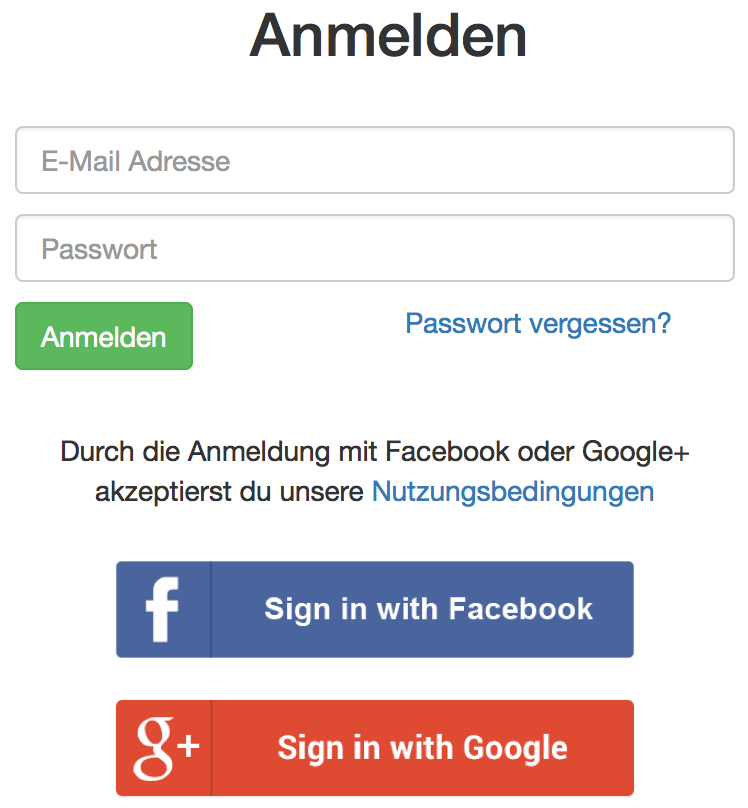
\includegraphics[width=0.35\textwidth]{images/usermanagement/Anmelden}
	\caption{Klassische Anmeldung oder mittels OAuth}
	\label{fig3}
\end{figure}

Um einen Benutzer anzumelden, muss zunächst ein User-Objekt mit der übergebenen Email Adresse von der Datenbank abgefragt werden. Sollte diese E-Mail Adresse keinem Benutzer zugeordnet sein, existiert der Benutzer noch nicht. Ansonsten muss mit \textit{.check\_password(...)} das eingegebene Passwort überprüft werden. Sollte dieses korrekt sein, kann der User angemeldet werden. Dazu muss das Authentication-Backend und ein Session Timeout gesetzt werden und der Benutzer über die Funktion \textit{login()} eingeloggt werden:
\begin{lstlisting}
try:
    user = User.objects.get(email='exampleATexample.com')
except:
    user = None
if user is not None and user.check_password('myPassword'):
    user.backend = 'mongoengine.django.auth.MongoEngineBackend'
    login(request, user)
    request.session.set_expiry(60 * 60 * 1) # 1 hour timeout
\end{lstlisting}

Der aktuell angemeldete Benutzer kann mittels \textit{request.user} abgefragt werden. Sollte der Benutzer aktuell nicht angemeldet sein, ist dies null, ansonsten wird das entsprechende User-Objekt zurückgeliefert.
Um einen angemeldeten Benutzer wieder abzumelden muss lediglich folgende Funktion ausgeführt werden:
\textit{logout(request)}

\subsubsection{Usersicht}

\begin{figure}[ht]
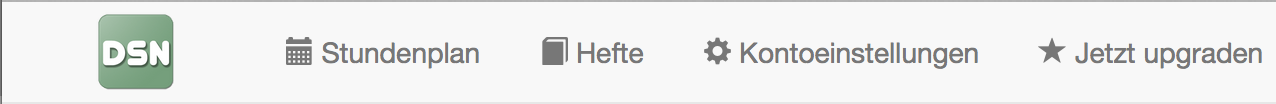
\includegraphics[width=0.85\textwidth]{images/usermanagement/Usersicht}
	\caption{Navigationsleiste als User}
	\label{fig4}
\end{figure}

Ein angemeldeter Benutzer kann seine Benutzerinformationen nachgiebig unter Kontoeinstellungen ändern. Für die Änderung seiner Daten, muss aus Sicherheitsgründen, dass aktuelle Passwort eingegeben werden.

\begin{figure}[ht]
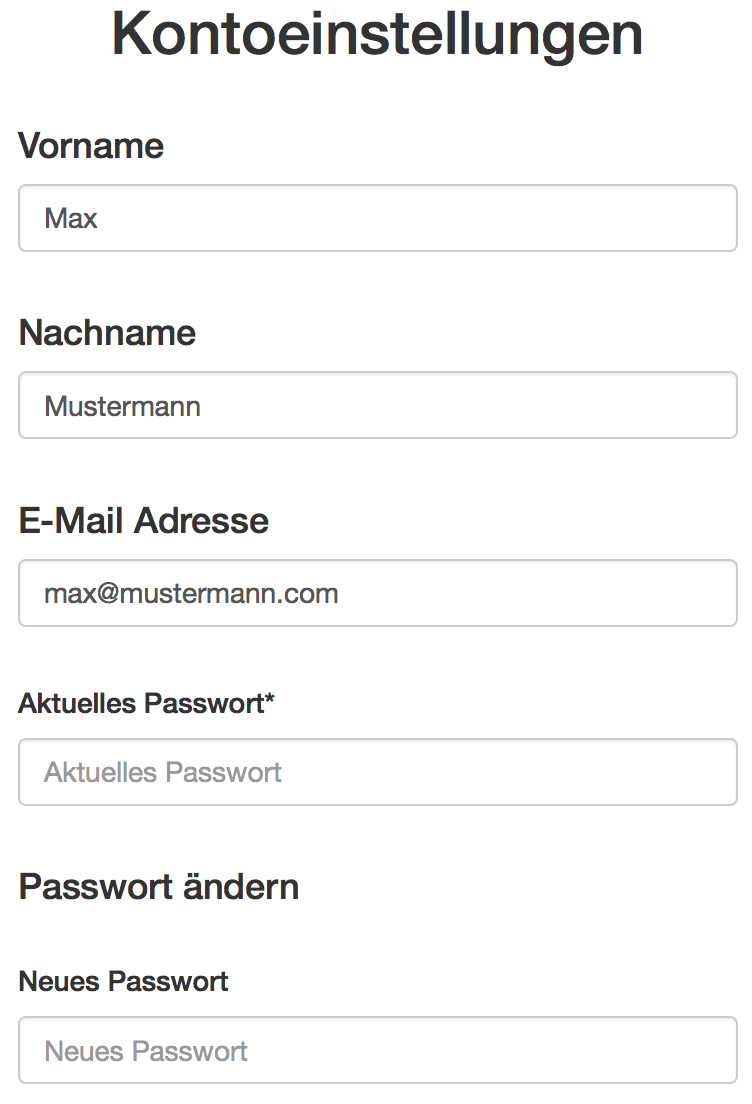
\includegraphics[width=0.35\textwidth]{images/usermanagement/Kontoeinstellungen}
	\caption{Kontoeinstellungen}
	\label{fig5}
\end{figure}

Im System befinden sich drei verschiedene Berechtigungsstufen, welche sind: der Standard-Benutzer, Pro-Benutzer und Administrator. Jedem/r registrierten AnwenderIn ist zu Beginn ein Standard-Benutzer. Ihnen stehen eine begrenzte Anzahl an digitalen Heften zur Verfügung. Durch eine geringe monatliche Zahlung kann der Standard-Account zum Pro-Account upgegradet werden, wodurch dem/r SchülerIn erweiterte Funktion angeboten werden. Zum einen stehen mehr Hefte zur Verfügung, es wird keine Werbung angezeigt, sowie keine Speicherbeschränkung. Die letzte Berechtigungsstufe sind Administratoren. Sie sind ebenfalls Pro-User, haben im Gegensatz einen eigenen Admin-Bereich, wo sämtliche Daten über Benutzer verwaltet und kontrolliert werden können. Dieser Bereich kann mit /admin nach der URL aufgerufen werden. Er unterscheidet sich durch den schwarzen Menübalken.\\
Jede/r BenutzerIn hat die Möglichkeit nach seinen Freunden oder anderen registrierten Anwendern zu suchen. Rechts oben in der Navigationleiste befindet sich ein Suchbalken, der es Anwendern ermöglicht nach Vornamen, Nachnamen oder nach Email-Adressen zu suchen.

\begin{figure}[ht]
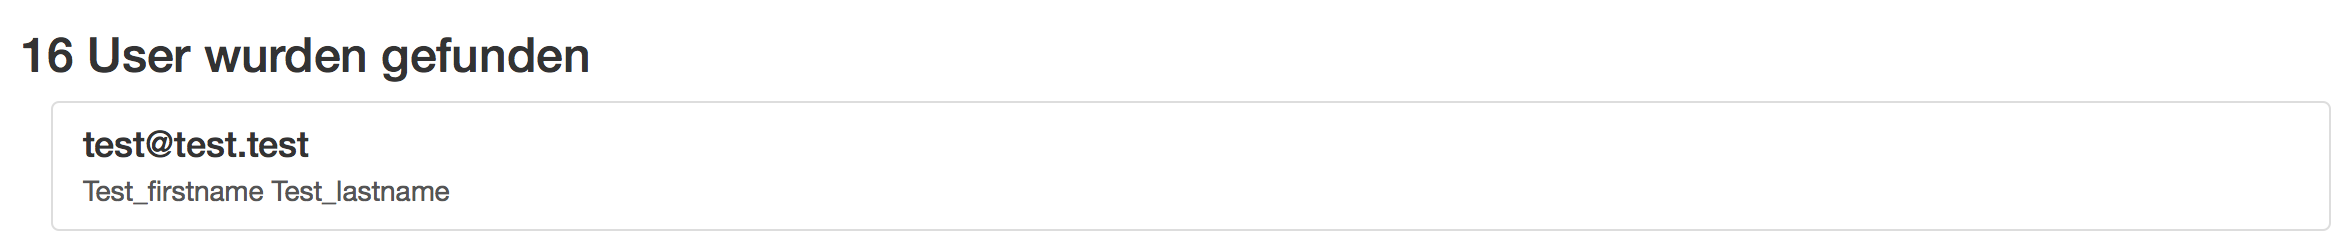
\includegraphics[width=0.85\textwidth]{images/usermanagement/Search}
	\caption{Usersuche}
	\label{fig6}
\end{figure}

Bei Klick auf den gefundenen User gelangt auf dessen Profil. Auf dem Profil ist zu einem der volle Name zu sehen, die Email-Adresse und die Berechtigungsstufe, ob es sich um einen Standardbenutzer, Pro-Benutzer oder Administrator handelt. Ein weiterer wichtiger Punkt sind die öffentlichen Hefte. Jeder User ist in der Lage von öffentlichen Heften andere einzelne Seiten zu exportieren.

\subsubsection{Adminsicht}


\includegraphics[width=0.35\textwidth]{images/usermanagement/Adminsicht}\\

Auf der User Management Page werden alle Benutzer von DSN aufgelistet. Man hat Einsicht auf die Email-Adresse, Vorname, Nachname und auf die Berechtigungsstufe, Standard-Benutzer, Pro-Benutzer, Administrator. Außerdem besteht die Möglichkeit als Administrator andere Benutzer zu löschen, die Berechtigungsstufe zu ändern oder den Benutzer mittels einer Mail auf etwas hinzuweisen. Neben der Auflistung der Benutzer, kann auch nach einer bestimmten Person suchen. Die Eingabe wird mit den Vorname, Nachnamen und der Email-Adresse verglichen. Mittels \textit{collectionName.objects()} liefert Mongoengine alle Objekte von der angegeben Collection. Wenn der Adminstrator aber nicht alle Objekte von einer Collection haben möchte, sondern nur eine gewisse Anzahl, können diese mit folgenden Befehl abgefragt werden:\textit{Tabellenname.objects[x:y]}\\
Objekte können wie folgt gesucht werden:\\
\textit{users(Q(email\_\_icontains=suchtext) \big| Q(first\_name\_\_icontains=suchtext) \big|\\
Q(last\_name\_\_icontains=suchtext))}\\
\\
Objekte können auch nach einer bestimmten Spalte sortiert werden.\\
\textit{users.order\_by(spaltenname)
users.order\_by('- '+spaltenname)}\\
\\
Falls man ein vorhandenes Objekt aus der Collection löschen möchte, muss dieses zuvor rausfiltern und dann mit der Funktion \textit{delete()} entfernen. Veränderte Daten werden mit der Funktion \textit{save()} persistiert.

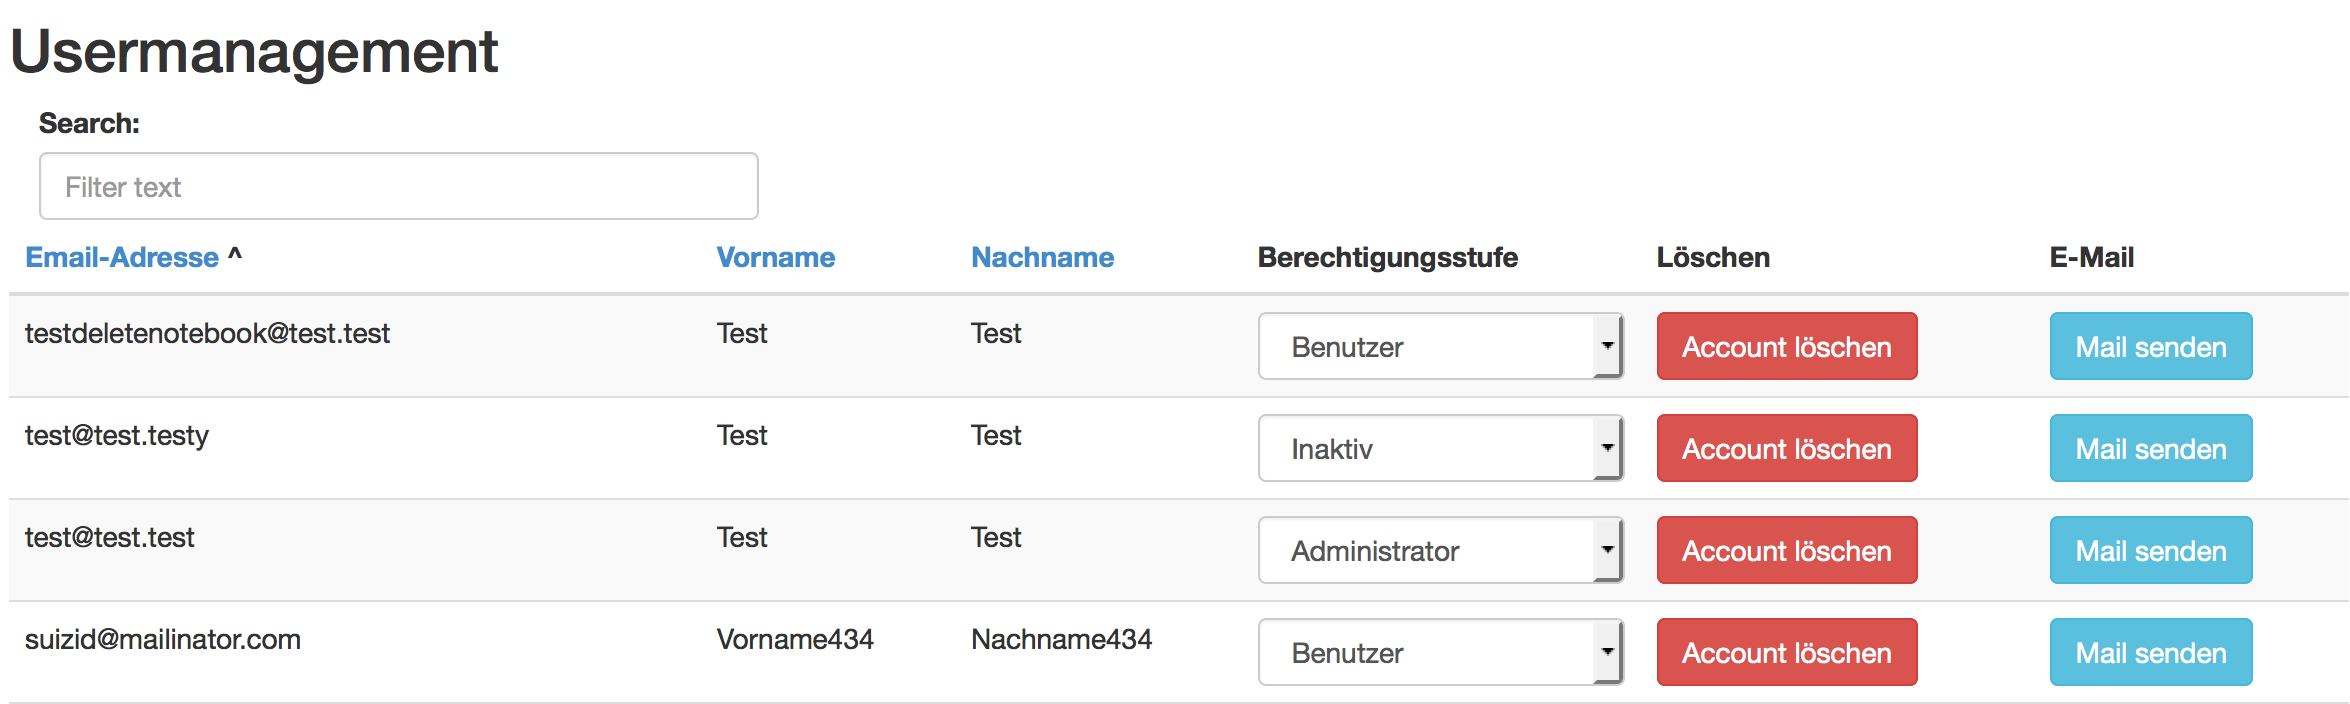
\includegraphics[width=0.65\textwidth]{images/usermanagement/Usermanagment}\\

Da unser User Management Page nur Seitenweise die Benutzerliefert, um Ladezeiten zu minimieren, muss diese mittels Pagination umgesetzt werden. Für die Realisierung sind die Anzahl der Objekte die insgesamt ausgegeben werden sollen gefordert. Dann wird definiert, wieviele Elemente pro Seite angezeigt werden sollen. Um die Seitenanzahl zu berechnen,  werden alle Elemente durch die Anzahl der Elemente dividiert, die pro Seite dargestellt werden sollen. Der Server übergibt dann die Elemente, welche auf einer Seite angezeigt werden sollen. Falls der User auf eine andere Seite wechselt, werden die nächsten Objekte vom Server bezogen.
\begin{lstlisting}
$http({
        method: 'GET',
        url: '/api/admin_user',
        data: {}
    })
        .success(function (data) {
            $scope.users = data['test'];
            $scope.len = data['len'];
            $scope.currentPage = 0;
            $scope.l = Math.ceil($scope.len/$scope.itemsPerPage);
        })
        .error(function (data) {
  });
    var searchMatch = function (haystack, needle) {
        if (!needle) {
            return true;
        }
        return haystack.toLowerCase().indexOf(needle.toLowerCase()) !== -1;
    };

    $scope.range = function (size, start, end) {
        var ret = [];
        if (size < end) {
            end = size;
            start = size;
        }
        for (var i = start; i < end; i++) {
            ret.push(i);
        }
        return ret;
    };

    $scope.firstPage = function () {
        $scope.currentPage = 0;
    };

    $scope.prevPage = function () {
        if ($scope.currentPage > 0) {
            $scope.currentPage--;
        }
    };

    $scope.nextPage = function () {
        if ($scope.currentPage < $scope.l- 1) {
            $scope.currentPage++;
        }
    };

    $scope.lastPage = function () {
        $scope.currentPage = $scope.l-1;
    };

    $scope.setPage = function () {
        $scope.currentPage = this.n;
    };

\end{lstlisting}

\begin{lstlisting}
def view_users(request):
    if not request.user.is_authenticated() or not request.user.is_superuser:
        return JsonResponse({})
    u = []
    length = 0
    weiter = False
    delete = False
    if request.method == "GET":
        users = User.objects[0:20]
        length = len(User.objects)
    elif request.method == "POST":
        params = json.loads(request.body.decode('utf-8'))
        von = (params['Page']-1)*params['counter']
        bis = params['counter']*params['Page']

        try:
            """ Delete """
            user = User.objects.get(email=params['email'])

            if user != request.user and user.delete_date == None:
                enddate = datetime.now() + timedelta(days=7)
                until = date(enddate.year, enddate.month, enddate.day)
                user.delete_date = until
                user.save()
                deleteemail(user.email, user.first_name, until)
            elif user != request.user:
                user.delete_date = None
                user.save()
        except KeyError:
            pass

        users = User.objects()

        try:
            """ Search """
            if bool(params['text'] and params['text'].strip()):
                users = users(Q(email__icontains=params['text']) | Q(first_name__icontains=params['text']) | Q(last_name__icontains=params['text']))
        except KeyError:
            pass

        try:
            """ Sort """
            if params['order'] is not None:
                if params['order']:
                    users = users.order_by(params['spalte'])
                else:
                    users = users.order_by('-'+str(params['spalte']))
        except KeyError:
            pass
        length = len(users)
        users = users[von:bis]
    for user in users:
        security = 1
        if user.is_prouser: security = 2
        if user.is_superuser: security = 3
        if not user.is_active: security = 4
        if user.delete_date == None:
            delete_state = 'Account loeschen'
        else:
            days = abs(datetime.today().day - int(date.strftime(user.delete_date, "%d")))
            delete_state = ' Loeschung in %s Tagen' % (str(days))

        u.append({
            "email": user.email,
            "first_name": user.first_name,
            "last_name": user.last_name,
            "security_level": security,
            "delete_account": delete_state
        })
    if length == 0:
        return JsonResponse({'test': u})
    else:
        return JsonResponse({'test': u, 'len': length})
\end{lstlisting}

Falls ein Pro-User seinen Zahlungen nicht nachkommt oder sich durch Böswilligkeiten bemerkbar macht hat der Administrator von DSN das Recht diesen User zu löschen. DSN gibt den User die Möglichkeit seine Daten bzw. Hefte bevor er gelöscht wird zu sichern. Der zu löschende Benutzer empfängt eine Email, wo darauf hingewiesen wird das sein Account und alle dazugehörigen Daten nach 7 Tagen gelöscht werden. Am Server von DSN läuft ein cronjob welcher jeden Tag das definierte Command, welches überprüft wann der zu löschende User entfernt werden soll, ausführt. Im Falle das jemand länger als 3 Monate interaktiv ist, wird ihm eine Informationsmail zugesendet. Diese informiert ihn, dass er sich in den 7 kommenden Tagen einloggen soll, ansonsten wird der Account mit alle den Daten gelöscht. \cite{COMMANDS}\cite{CRON}

\begin{lstlisting}
from django.core.management import BaseCommand
from datetime import *
from dsn.models import User
from dsn.authentication.account_delete import delete_account

#https://docs.djangoproject.com/en/1.9/howto/custom-management-commands/
#The class must be named Command, and subclass BaseCommand
class Command(BaseCommand):
    # Show this when the user types help
    help = "Command for the User notification"

    # A command must define handle()
    def handle(self, *args, **options):
        until = datetime.now() + timedelta(days=7)
        users = User.objects(delete_date__lte=until)
        for user in users:
            now = datetime.today()
            day = abs(now.day - int(date.strftime(user.delete_date, "%d")))
            if day == 0:#User delete
                delete_account(user)
\end{lstlisting}

Cronjob
\begin{lstlisting}
# m h  dom mon dow   command
# * *   */1   *   *    python3 /home/stable/dsn/manage.py inform
# * *   */1   *   *    python3 /home/stable/dsn/manage.py delete
\end{lstlisting}

Unter dem Navigationspunkt Bills werden die Rechnungen von den Pro-Benutzern aufgelistet. Zum einen wann und ob der Betrag eingezahlt wurde.